\chapter{Opis projektnog zadatka}
		
		
		Cilj ovog projekta je razvoj i implementacija aplikacije Digitaliziraj, koja će tvrtkama olakšati digitalizaciju dokumenata nužnih za poslovanje koristeći OCD (eng. Optical character recognition). Aplikacija će olakšati digitalizaciju dokumenata unutar organizacija, te osigurati da svaki radnik organizacije dobije dokumente za koje je zadužen. Time, aplikacija će povećati učinkovitost organizacije te ubrzati njeno djelovanje.\\
		
		Neregistrirani korisnik mora napraviti korisnički račun kako bi mogao koristiti funkcionalnosti aplikacije. Za to su mu potrebni sljedeći podatci:
		
		\begin{packed_item}
			\item \textit{ime}
			\item \textit{prezime}
			\item \textit{email adresa}
			\item \textit{lozinka}
		\end{packed_item}
	
	Dodatno, ne registrirani korisnik mora odabrati na kojoj razini ovlasti želi stvoriti korisnički račun. Dostupne su 4 razine ovlasti:
	
	\begin{packed_item}
		\item \textit{zaposlenik}
		\item \textit{revizor}
		\item \textit{računovođa}
	\end{packed_item}
	
	Razne razine iznad su navedene od najniže do najviše. U većini slučajeva viša razina ovlasti ima sve funkcionalnosti onih ispod sebe, osim u onim slučajevima kada struktura tvrtke te razne odgovornosti zaposlenika to traže drugačije. Detalji o funkcionalnostima svake razine ovlasti nalaze se u nastavku dokumenta. Dodatno postoji još razina ovlasti direktor, koja predstavlja razinu ovlasti vlasnika tvrtke. Aplikacija sama stvara jedan korisnički račun s tom razinom ovlasti te su podatci potrebni za prijavu u taj korisnički račun dani vlasniku tvrtke.\\
	
	Zaposlenik ima najnižu razinu ovlasti unutar sustava. Korisnik s razinom ovlasti zaposlenik može učitavati slike u sustav te provjeriti jeli sustav točno odradio konverziju slike u dokument. Jednom kad zaposlenik potvrdi da je pretvorba iz slike u dokument odrađena ispravno, generiran dokument se šalje jednom od revizora tvrtke na pregled. U svrhu ubrzanja procesa aplikacija omogućuje učitavanje do 50 slika istovremeno (ova funkcionalnost omogućena je i za sve više razine ovlasti). Pri tom zaposlenik i dalje mora svaku od konverzija potvrditi kao točnu prije nego što je dokument proslijeđen revizoru na pregled. Zaposlenik ima pristup povijesti svih dokumenata koje je skenirao.\\
	
	Revizor je druga najniža razina ovlasti unutar sustava. Posao revizora jest kontrola rada zaposlenika te preusmjeravanje dokumenata odgovarajućem računovođi (ovisno o vrsti dokumenta). Kao takav revizor ima pristup povijesti svih dokumenata nad kojima je vršio kontrolu. U slučaju da revizor skenira dokument aplikacija će automatski detektirati računovođu kojem vrsta skeniranog dokumenta treba biti poslana, te će nakon što revizor potvrdi ispravnost konverzije taj dokument biti automatski poslan odgovarajućem računovođi.\\
	
	
	Računovođa je najviša razina ovlasti u sustavu, izuzev direktora. Svaki računovođa je zadužen za obradu jedne od 3 vrste dokumenata koje aplikacija raspoznaje. To su računi, ponude i interni dokumenti. Računovođa ima pristup povijesti svih dokumenata one vrste za koju je zadužen. Posao računovođe je arhivirati dokumente. Pri arhiviranju dokumentu se dodjeljuje jedinstven broj arhiva. Računovođa također po potrebi može poslati dokument direktoru na potpisivanje. U tom slučaju direktor prima obavijest o tome. Nakon što direktor potpiše dokument računovođa dobiva obavijest da je dokument potpisan te ga onda može arhivirati. U slučaju da računovođa učita sliku dokumenta one vrste za koju nije zadužen aplikacija će mu automatski ponuditi slanje dokumenta odgovarajućem računovođi.\\
	
	Direktor je najviša razina ovlasti unutar sustava, te predstavlja najodgovorniju osoba unutar organizacije koja koristi aplikaciju za svoje poslovanje. Direktor ima uvid u povijest svih dokumenata te u statistike svih zaposlenika. U slučaju da mu računovođa pošalje zahtjev za potpis može potpisati dokument. U slučaju da direktor sam učitava slike u sustav te vrši konverziju, odmah mu se nudi mogućnost potpisivanja dokumenta te aplikacija automatski određuje računovođu kojem treba proslijediti učitan dokument. Dodatno za promotivne svrhe, direktoru je omogućena objava dokumenata na sljedećim društvenim mrežama: (???treba dodati koje društvene mreže jednom kad ustanovimo koje ćemo društvene vježbe koristiti) \\
	
	\section{Potencijalna korist ovog projekta}
	
	Svojom strukturom i funkcionalnošću aplikacija ostvaruje brz i učinkovit sustav digitalizacije i distribucije dokumenata unutar organizacije. Njenom primjenom može se osigurati učinkovito poslovanje te raspodjela odgovornosti među zaposlenicima što pospješuje rad organizacije u mnogim aspektima. S obzirom na njenu općenitost aplikacija bi mogla biti  od interesa svim organizacijama koje se moraju baviti papirologijom. To uključuje: neprofitne humanitarne organizacije, tvrtke koje se natječu na tržištu, vladine agencije...\\
	
	\section{Slična rješenja}
	
	Na tržištu postoje razni sustavi za distribuciju dokumenata (???), također postoje i mnoge implementacije OCR-a.(???) No vrlo je malen broj alata koji integriraju te dvije tehnologije u jedan sustav. Time se zaobilazi potreba da se odvojeni alati koriste za digitalizaciju dokumenata i njihovu distribuciju. (Treba dodati imena i slike koje se traže)\\
	
	\section{Mogućnost prilagodbe}
	
	Implementacija sustava u velikoj mjeri ovisi o strukturi organizacije i njenim potrebama za distribuciju dokumenata. Dodatno ako je klasifikacija dokumenata koju organizacija koristi složenija, potrebno je doraditi sustav automatskog prosljeđivanja dokumenata. Međutim implementacija djelova sustava, koji se ne moraju mijenjati ovisno o potrebi klijenta, mogu se izvesti na način da je ta promjena relativno jednostavna.
	
	\section{Opseg projektnog zadatka}
	
	Konkretna implementacija izvedena u sklopu ovog projekta koristi relativno jednostavnu strukturu organizacije opisanu iznad, te razlikuje 4 različite vrste dokumenata. To je čini relativno jednostavnom za implementaciju no ujedno.
	
	\section{Moguće nadogradnje}
	
	Mnoge nadogradnje su moguće na sustav. Integracija s alatima za preuređivanje digitalnih dokumenata...
	
	
		
		\begin{packed_item}
			\item \textit{potencijalna korist ovog projekta}
			\item \textit{postojeća slična rješenja (istražiti i ukratko opisati razlike u odnosu na zadani zadatak). Dodajte slike koja predočavaju slična rješenja.}
			\item \textit{skup korisnika koji bi mogao biti zainteresiran za ostvareno rješenje.}
			\item \textit{mogućnost prilagodbe rješenja }
			\item \textit{opseg projektnog zadatka}
			\item \textit{moguće nadogradnje projektnog zadatka}
		\end{packed_item}
		
		\textit{Za pomoć pogledati reference navedene u poglavlju „Popis literature“, a po potrebi konzultirati sadržaj na internetu koji nudi dobre smjernice u tom pogledu.}
		\eject
		
		\section{Primjeri u \LaTeX u}
		
		\textit{Ovo potpoglavlje izbrisati.}\\

		U nastavku se nalaze različiti primjeri kako koristiti osnovne funkcionalnosti \LaTeX a koje su potrebne za izradu dokumentacije. Za dodatnu pomoć obratiti se asistentu na projektu ili potražiti upute na sljedećim web sjedištima:
		\begin{itemize}
			\item Upute za izradu diplomskog rada u \LaTeX u - \url{https://www.fer.unizg.hr/_download/repository/LaTeX-upute.pdf}
			\item \LaTeX\ projekt - \url{https://www.latex-project.org/help/}
			\item StackExchange za Tex - \url{https://tex.stackexchange.com/}\\
		
		\end{itemize} 	


		
		\noindent \underbar{podcrtani tekst}, \textbf{podebljani tekst}, 	\textit{nagnuti tekst}\\
		\noindent \normalsize primjer \large primjer \Large primjer \LARGE {primjer} \huge {primjer} \Huge primjer \normalsize
				
		\begin{packed_item}
			
			\item  primjer
			\item  primjer
			\item  primjer
			\item[] \begin{packed_enum}
				\item primjer
				\item[] \begin{packed_enum}
					\item[1.a] primjer
					\item[b] primjer
				\end{packed_enum}
				\item primjer
			\end{packed_enum}
			
		\end{packed_item}
		
		\noindent primjer url-a: \url{https://www.fer.unizg.hr/predmet/proinz/projekt}
		
		\noindent posebni znakovi: \# \$ \% \& \{ \} \_ 
		$|$ $<$ $>$ 
		\^{} 
		\~{} 
		$\backslash$ 
		
		
		\begin{longtblr}[
			label=none,
			entry=none
			]{
				width = \textwidth,
				colspec={|X[8,l]|X[8, l]|X[16, l]|}, 
				rowhead = 1,
			} %definicija širine tablice, širine stupaca, poravnanje i broja redaka naslova tablice
			\hline \SetCell[c=3]{c}{\textbf{naslov unutar tablice}}	 \\ \hline[3pt]
			\SetCell{LightGreen}IDKorisnik & INT	&  	Lorem ipsum dolor sit amet, consectetur adipiscing elit, sed do eiusmod  	\\ \hline
			korisnickoIme	& VARCHAR &   	\\ \hline 
			email & VARCHAR &   \\ \hline 
			ime & VARCHAR	&  		\\ \hline 
			\SetCell{LightBlue} primjer	& VARCHAR &   	\\ \hline 
		\end{longtblr}
		

		\begin{longtblr}[
				caption = {Naslov s referencom izvan tablice},
				entry = {Short Caption},
			]{
				width = \textwidth, 
				colspec = {|X[8,l]|X[8,l]|X[16,l]|}, 
				rowhead = 1,
			}
			\hline
			\SetCell{LightGreen}IDKorisnik & INT	&  	Lorem ipsum dolor sit amet, consectetur adipiscing elit, sed do eiusmod  	\\ \hline
			korisnickoIme	& VARCHAR &   	\\ \hline 
			email & VARCHAR &   \\ \hline 
			ime & VARCHAR	&  		\\ \hline 
			\SetCell{LightBlue} primjer	& VARCHAR &   	\\ \hline 
		\end{longtblr}
	


		
		
		%unos slike
		\begin{figure}[H]
			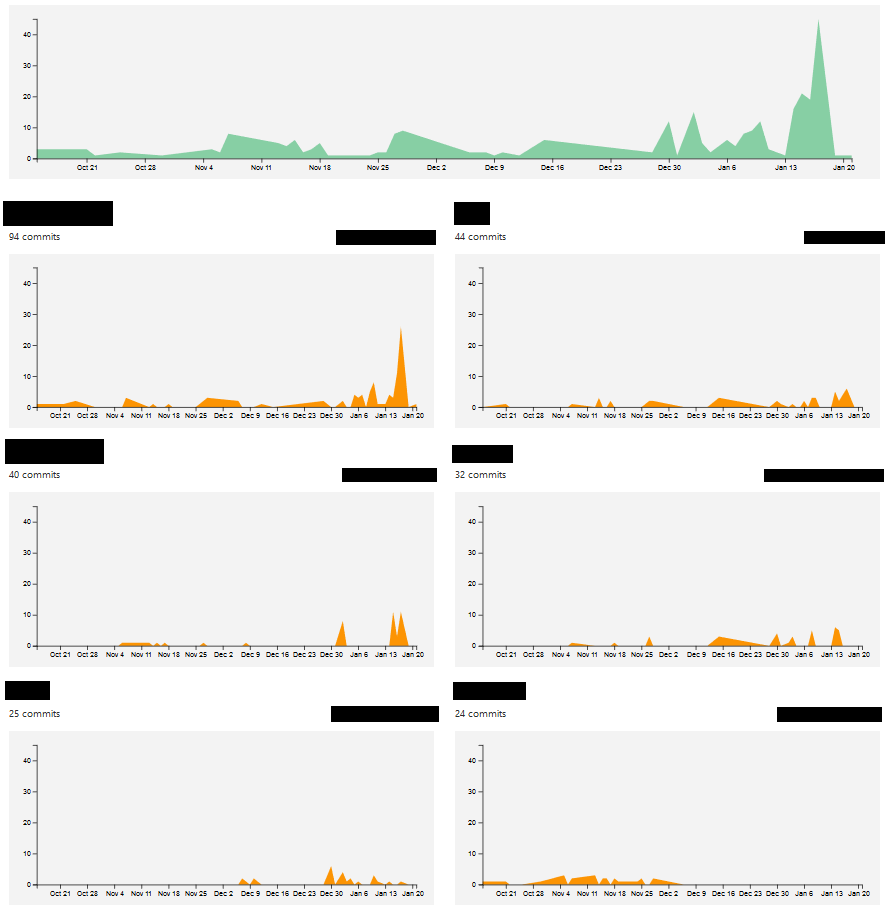
\includegraphics[scale=0.4]{slike/aktivnost.PNG} %veličina slike u odnosu na originalnu datoteku i pozicija slike
			\centering
			\caption{Primjer slike s potpisom}
			\label{fig:promjene}
		\end{figure}
		
		\begin{figure}[H]
			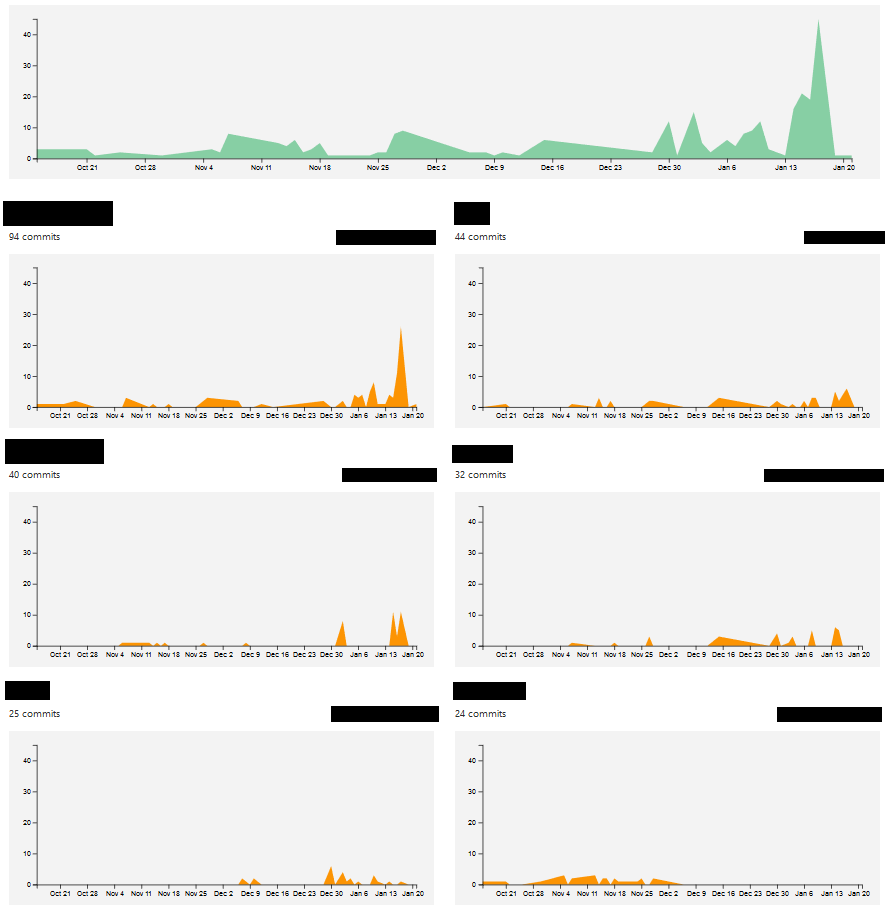
\includegraphics[width=\textwidth]{slike/aktivnost.PNG} %veličina u odnosu na širinu linije
			\caption{Primjer slike s potpisom 2}
			\label{fig:promjene2} %label mora biti drugaciji za svaku sliku
		\end{figure}
		
		Referenciranje slike \ref{fig:promjene2} u tekstu.
		
		\eject
		
	